\documentclass[12pt,a4paper]{article}
\usepackage[utf8]{inputenc}
\usepackage[T1]{fontenc}
\usepackage[margin=1in]{geometry}
\usepackage{hyperref}
\usepackage{graphicx}
\usepackage{tikz}
\usepackage{enumitem}
\usepackage{array}
\usepackage{longtable}
\usepackage{booktabs}
\usepackage{amsmath}
\usepackage{amsfonts}
\usepackage{setspace}
\usepackage{longtable}
\usepackage{makecell}   % for \makecell{..\\..}
\makegapedcells
\usepackage{tabularx}   
% Configure hyperref for blue links in TOC
\hypersetup{
    colorlinks=true,
    linkcolor=blue,
    filecolor=blue,
    urlcolor=blue,
    citecolor=blue,
}

% TikZ libraries for figures
\usetikzlibrary{shapes,arrows,positioning,shadows}

% Line spacing
\onehalfspacing

% Custom commands for consistency
\newcommand{\sectionbreak}{\vspace{0.5cm}}
\newcommand{\subsectionbreak}{\vspace{0.3cm}}





\begin{document}
\input{titlepage}

\newpage

\tableofcontents

\newpage

\section{Project Overview}

 The main goal of the Healthcare Web Application is to make healthcare management easier by letting people access medical records, schedule appointments, and communicate with healthcare providers. The application connects patients, doctors, and administrators in one structured system.\\
\noindent
The system has three types of users:
\begin{itemize}[itemsep=0.2cm]
    \item \textbf{Patients} - manage their health information and book appointments
    \item \textbf{Doctors} - view patient records and manage their schedule
    \item \textbf{Administrators} - manage user accounts and system settings
\end{itemize}

We will use agile development over 12 weeks to build the app in small steps and receive feedback regularly to make sure we are on the right track.

\sectionbreak

\section{Functional Requirements}

\subsection{User Authentication and Login}

The system needs secure login for three types of users: patients, doctors, and administrators. Each user type can only access the parts of the system they need. Key features include,
\begin{itemize}[itemsep=0.1cm]
    \item User registration with email confirmation
    \item Secure login and logout
    \item Password reset through email
    \item Account management (update profile, change password)
    \item Different access levels for each user type
\end{itemize}

\subsection{Patient Features}
\begin{enumerate}
    \item 
        \textbf{Profile Management}
        \begin{itemize}[itemsep=0.1cm]
            \item Create and update personal information
            \item Add emergency contact details
            \item Manage basic medical information
        \end{itemize}

    \item 
        \textbf{Medical History}
        \begin{itemize}[itemsep=0.1cm]
            \item View past appointments and treatments
            \item See prescription history
            \item Access test results and doctor notes
        \end{itemize}
    \item 
        \textbf{Appointment Booking}
        \begin{itemize}[itemsep=0.1cm]
            \item View available doctors and time slots
            \item Book appointments online
            \item Cancel or reschedule appointments
            \item Get appointment reminders
        \end{itemize}
        
\end{enumerate}





\subsection{Doctor Features}

\begin{enumerate}
    \item 
\textbf{Patient Management}
\begin{itemize}[itemsep=0.1cm]
    \item View list of assigned patients
    \item Access patient medical history
    \item Review upcoming appointments
\end{itemize}
    \item 
\textbf{Schedule Management}
\begin{itemize}[itemsep=0.1cm]
    \item See daily and weekly appointment schedule
    \item Update appointment status
    \item Add notes after patient visits
\end{itemize}
    \item 
\textbf{Prescription Management}
\begin{itemize}[itemsep=0.1cm]
    \item Create new prescriptions
    \item Update existing medications
    \item View patient's current prescriptions
\end{itemize}
\end{enumerate}







\subsection{Administrator Features}

\begin{enumerate}
    \item 
\textbf{User Management}
\begin{itemize}[itemsep=0.1cm]
    \item Create, edit, and deactivate user accounts
    \item Assign roles to users (patient, doctor, admin)
    \item Reset user passwords when needed
\end{itemize}
    \item 
\textbf{System Monitoring}
\begin{itemize}[itemsep=0.1cm]
    \item View basic usage statistics
    \item Monitor system activity
    \item Generate simple reports
\end{itemize}
    \item 
\textbf{System Settings}
\begin{itemize}[itemsep=0.1cm]
    \item Configure appointment time slots
    \item Set up system notifications
    \item Manage basic application settings
\end{itemize}
\end{enumerate}







\subsection{Additional Features}
\begin{enumerate}
    \item 
\textbf{Medical imaging upload and viewing}
\begin{itemize}[itemsep=0.1cm]
    \item Medical documents(PDF, images) can be uploaded to the system
    \item Doctors can view uploaded files securely
\end{itemize}

    \item 
\textbf{Medication tracking and reminders}
\begin{itemize}[itemsep=0.1cm]
    \item Reminder system for taking medications
    \item Display current prescriptions
    \item Notification for refills
\end{itemize}
\end{enumerate}



\sectionbreak

\section{Non-Functional Requirements}

\subsection{Security}

The application must protect patient information and prevent unauthorized access:

\begin{itemize}[itemsep=0.1cm]
    \item All data sent between browser and server is encrypted (HTTPS)
    \item User passwords are stored securely
    \item Input validation to prevent common attacks
    \item Session management with automatic logout
    \item Basic protection of sensitive patient data
\end{itemize}

\subsection{Performance}

The system should work well under normal use:

\begin{itemize}[itemsep=0.1cm]
    \item Pages load within reasonable time
    \item Support multiple users at the same time
    \item Basic database optimization for faster searches
    \item Efficient file uploads and downloads
\end{itemize}

\subsection{Reliability}

The system should work consistently:

\begin{itemize}[itemsep=0.1cm]
    \item Basic error handling with helpful messages
    \item Regular data backups
    \item System logging for troubleshooting
    \item Stable operation under normal conditions
\end{itemize}

\sectionbreak

\section{User Stories with Acceptance Criteria}

\subsection{Patient-User Stories}

\begin{figure}[h!]
\centering
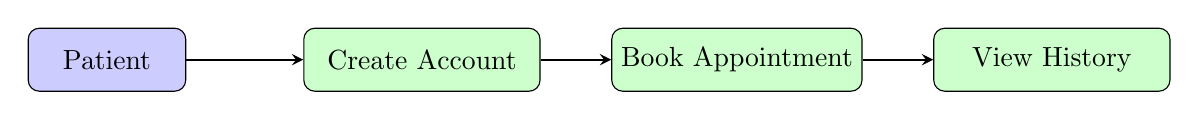
\begin{tikzpicture}[node distance=2cm, auto]
    % Define styles
    \tikzstyle{user} = [rectangle, rounded corners, minimum width=2cm, minimum height=0.8cm, text centered, draw=black, fill=blue!20]
    \tikzstyle{action} = [rectangle, rounded corners, minimum width=3cm, minimum height=0.8cm, text centered, draw=black, fill=green!20]
    \tikzstyle{arrow} = [thick,->,>=stealth]
    
    % Nodes
    \node [user] (patient) {Patient};
    \node [action, right of=patient, xshift=2cm] (register) {Create Account};
    \node [action, right of=register, xshift=2cm] (book) {Book Appointment};
    \node [action, right of=book, xshift=2cm] (history) {View History};
    
    % Arrows
    \draw [arrow] (patient) -- (register);
    \draw [arrow] (register) -- (book);
    \draw [arrow] (book) -- (history);
\end{tikzpicture}
\caption{Patient-User Journey}
\label{fig:patient_journey}
\end{figure}
\noindent
\subsubsection{Story 1: Account Creation}
\begin{center}
    \textit{"As a patient, I want to create an account so I can use the healthcare system."}
\end{center}


Acceptance Criteria:
\begin{itemize}[itemsep=0.1cm]
    \item Registration form with required fields works correctly
    \item Email verification is sent and works
    \item User can log in with new account
    \item Profile information can be updated after registration
\end{itemize}

\subsubsection{Story 2: Appointment Booking}

\begin{center}
    \textit{"As a patient, I want to schedule appointments with doctors online."}
\end{center}

Acceptance Criteria:
\begin{itemize}[itemsep=0.1cm]
    \item Available time slots are shown clearly
    \item Booking process is simple and works
    \item Confirmation is sent after booking
    \item Appointments appear in my schedule
\end{itemize}

\subsubsection{Story 3: Medical History Access}

\begin{center}
    \textit{"As a patient, I want to see my medical history to track my health."}
\end{center}

Acceptance Criteria:
\begin{itemize}[itemsep=0.1cm]
    \item Medical history is displayed in chronological order
    \item Information is easy to read and understand
    \item Past prescriptions and treatments are shown
    \item Data loads quickly when requested
\end{itemize}

\subsection{Doctor-User Stories}

\begin{figure}[h!]
\centering
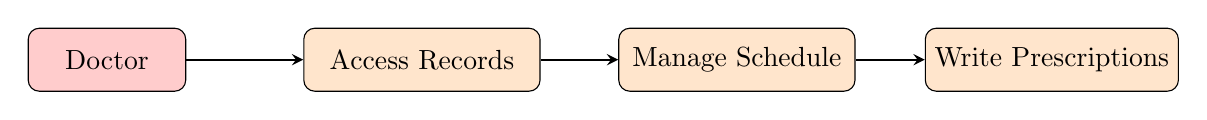
\begin{tikzpicture}[node distance=2cm, auto]
    % Define styles
    \tikzstyle{user} = [rectangle, rounded corners, minimum width=2cm, minimum height=0.8cm, text centered, draw=black, fill=red!20]
    \tikzstyle{action} = [rectangle, rounded corners, minimum width=3cm, minimum height=0.8cm, text centered, draw=black, fill=orange!20]
    \tikzstyle{arrow} = [thick,->,>=stealth]
    
    % Nodes
    \node [user] (doctor) {Doctor};
    \node [action, right of=doctor, xshift=2cm] (records) {Access Records};
    \node [action, right of=records, xshift=2cm] (schedule) {Manage Schedule};
    \node [action, right of=schedule, xshift=2cm] (prescribe) {Write Prescriptions};
    
    % Arrows
    \draw [arrow] (doctor) -- (records);
    \draw [arrow] (records) -- (schedule);
    \draw [arrow] (schedule) -- (prescribe);
\end{tikzpicture}
\caption{Doctor-User Journey}
\label{fig:doctor_journey}
\end{figure}

\subsubsection{Story 1: Patient Record Access}

\begin{center}
    \textit{"As a doctor, I need to view patient records to provide good care."}
\end{center}

Acceptance Criteria:
\begin{itemize}[itemsep=0.1cm]
    \item Patient list is easy to navigate
    \item Complete medical history loads properly
    \item Current medications are clearly displayed
    \item Information is organized and readable
\end{itemize}

\subsubsection{Story 2: Schedule Management}

\begin{center}
    \textit{"As a doctor, I want to manage my appointments efficiently."}
\end{center}

Acceptance Criteria:
\begin{itemize}[itemsep=0.1cm]
    \item Daily and weekly calendar views work
    \item Patient information is easily accessible
    \item Appointment details are clear
    \item Schedule updates work properly
\end{itemize}

\subsubsection{Story 3: Prescription Writing}

\begin{center}
    \textit{"As a doctor, I need to create prescriptions for patients."}

\end{center}

Acceptance Criteria:
\begin{itemize}[itemsep=0.1cm]
    \item Prescription form is easy to use
    \item Patient medication history is available
    \item New prescriptions are saved correctly
    \item Prescription list updates properly
\end{itemize}

\subsection{Administrator-User Stories}

\begin{figure}[h!]
\centering
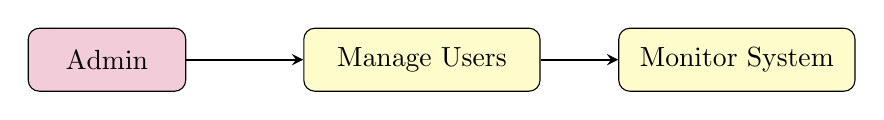
\begin{tikzpicture}[node distance=2cm, auto]
    % Define styles
    \tikzstyle{user} = [rectangle, rounded corners, minimum width=2cm, minimum height=0.8cm, text centered, draw=black, fill=purple!20]
    \tikzstyle{action} = [rectangle, rounded corners, minimum width=3cm, minimum height=0.8cm, text centered, draw=black, fill=yellow!20]
    \tikzstyle{arrow} = [thick,->,>=stealth]
    
    % Nodes
    \node [user] (admin) {Admin};
    \node [action, right of=admin, xshift=2cm] (users) {Manage Users};
    \node [action, right of=users, xshift=2cm] (monitor) {Monitor System};
    
    % Arrows
    \draw [arrow] (admin) -- (users);
    \draw [arrow] (users) -- (monitor);
\end{tikzpicture}
\caption{Administrator-User Journey}
\label{fig:admin_journey}
\end{figure}

\subsubsection{Story 1: User Management}

\begin{center}
    \textit{"As an administrator, I need to manage user accounts for security."}

\end{center}

Acceptance Criteria:
\begin{itemize}[itemsep=0.1cm]
    \item All user accounts are displayed with their roles
    \item New accounts can be created successfully
    \item Account information can be edited
    \item Users can be deactivated when needed
\end{itemize}

\subsubsection{Story 2: System Monitoring}

\begin{center}
    \textit{"As an administrator, I want to monitor system usage."}

\end{center}

Acceptance Criteria:
\begin{itemize}[itemsep=0.1cm]
    \item Basic usage statistics are displayed
    \item User activity can be reviewed
    \item Simple reports can be generated
    \item Data is presented clearly
\end{itemize}

\sectionbreak

\section{Technology Stack Justification}

\begin{figure}[h!]
\centering
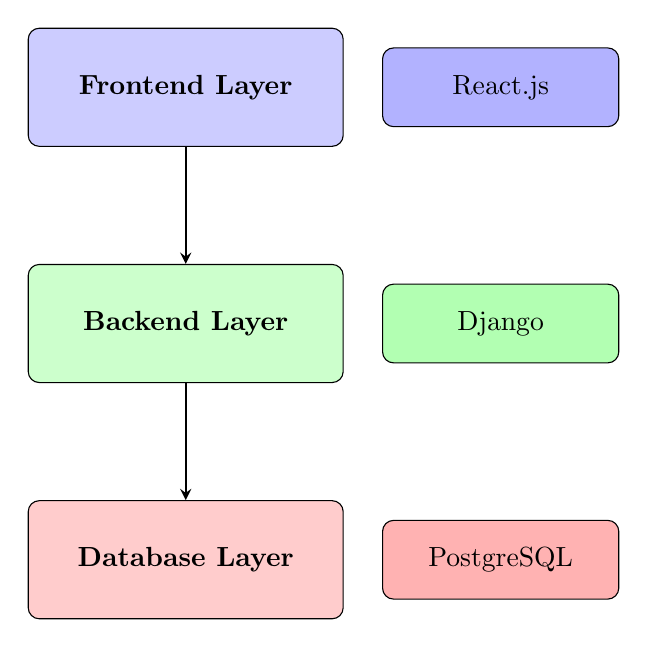
\begin{tikzpicture}[node distance=3cm, auto]
    % Define styles
    \tikzstyle{layer} = [rectangle, rounded corners, minimum width=4cm, minimum height=1.5cm, text centered, draw=black, fill=gray!10]
    \tikzstyle{tech} = [rectangle, rounded corners, minimum width=3cm, minimum height=1cm, text centered, draw=black]
    \tikzstyle{arrow} = [thick,->,>=stealth]
    
    % Layers
    \node [layer, fill=blue!20] (frontend) {\textbf{Frontend Layer}};
    \node [layer, fill=green!20, below of=frontend] (backend) {\textbf{Backend Layer}};
    \node [layer, fill=red!20, below of=backend] (database) {\textbf{Database Layer}};
    
    % Technologies
    \node [tech, fill=blue!30, right of=frontend, xshift=1cm] (react) {React.js};
    \node [tech, fill=green!30, right of=backend, xshift=1cm] (django) {Django};
    \node [tech, fill=red!30, right of=database, xshift=1cm] (postgres) {PostgreSQL};
    
    % Arrows
    \draw [arrow] (frontend) -- (backend);
    \draw [arrow] (backend) -- (database);
\end{tikzpicture}
\caption{Technology Stack Architecture}
\label{fig:tech_stack}
\end{figure}

\subsection{Backend: Django (Python)}

We chose Django because:
\begin{itemize}[itemsep=0.1cm]
    \item Built-in security features protect against common web attacks
    \item User authentication system works well for our three user types
    \item Good documentation and community support
    \item Handles database relationships effectively
    \item Django REST Framework makes API development easier
\end{itemize}

\subsection{Frontend: React.js}

We chose React because:
\begin{itemize}[itemsep=0.1cm]
    \item Component-based structure fits our different user interfaces
    \item Good for interactive features like appointment booking
    \item Large community with helpful resources
    \item Works well with Django APIs
    \item Team members have some experience with React
\end{itemize}

\subsection{Database: PostgreSQL}

We chose PostgreSQL because:
\begin{itemize}[itemsep=0.1cm]
    \item Reliable and handles complex data relationships
    \item Good performance for our expected usage
    \item Strong backup and recovery features
    \item Free and open-source
    \item Works well with Django
\end{itemize}


Our selected stack of Django, React, and PostgreSQL offers a coherent and practical solution for the healthcare application. Django provides a secure and structured backend with built-in authentication and ORM support, React delivers responsive and interactive interfaces for different user roles, and PostgreSQL ensures reliable handling of complex healthcare data. This combination not only supports our functional requirements such as appointment scheduling, prescription management, and medical record access, but also addresses non-functional needs like security, scalability, and performance. The technologies complement each other well, align with the project guidelines, and match the team’s skill set, allowing us to build a system that is both robust and achievable within the semester timeline.

\sectionbreak

\section{Team Roles and Responsibilities}

\subsection{Team Lead: Abu Ruhan Mahamud}
\textbf{Primary Responsibilities:}
\begin{itemize}[itemsep=0.1cm]
    \item Coordinate project activities and deadlines
    \item Manage communication between team members
    \item Plan sprint activities and track progress
    \item Handle project documentation and submissions
    \item Resolve conflicts and make final decisions
\end{itemize}

% \textbf{Secondary Tasks:}
% \begin{itemize}[itemsep=0.1cm]
%     \item Help with testing and quality assurance
%     \item Support other team members when needed
%     \item Maintain project management tools (Trello, Git)
% \end{itemize}

\subsection{Backend Developer: Md. Emranul Hoque}
\textbf{Primary Responsibilities:}
\begin{itemize}[itemsep=0.1cm]
    \item Develop Django application and APIs
    \item Design and implement database models
    \item Handle user authentication and security
    \item Set up deployment infrastructure
\end{itemize}

% \textbf{Secondary Tasks:}
% \begin{itemize}[itemsep=0.1cm]
%     \item Support frontend integration
%     \item Help with testing backend functionality
%     \item Assist with database optimization
% \end{itemize}

\subsection{Frontend Developer: Shahrukh Ahmed Meherab}
\textbf{Primary Responsibilities:}
\begin{itemize}[itemsep=0.1cm]
    \item Build React user interfaces for all user types
    \item Implement responsive design for different screen sizes
    \item Connect frontend to backend APIs
    \item Handle user experience and interface design
    \item Test frontend functionality across browsers
\end{itemize}

% \textbf{Secondary Tasks:}
% \begin{itemize}[itemsep=0.1cm]
%     \item Help with API design decisions
%     \item Support overall application testing
%     \item Assist with user documentation
% \end{itemize}

% \sectionbreak

\section{Project Timeline and Milestones}

\subsection{Major Deliverables}

\begin{longtable}{|p{3.25cm}|p{3.75cm}|p{7.5cm}|}
\hline
\textbf{Timeline} & \textbf{Deliverable} & \textbf{Description} \\
\hline
\endfirsthead

\hline
\textbf{Timeline} & \textbf{Deliverable} & \textbf{Description} \\
\hline
\endhead

\hline
\endfoot

\hline
\endlastfoot

\makecell[l]{Week 2\\(Sep 17, 2025)} & Requirements \& Setup & Complete requirements document, set up development environment, create project repository \\
\hline
\makecell[l]{Week 4\\(Oct 5, 2025)} & Design Documentation & Database design, API specifications, UI mockups, system architecture \\
\hline
\makecell[l]{Week 6\\(Oct 19, 2025)} & Backend Implementation & User authentication, core database models, basic API endpoints, testing framework \\
\hline
\makecell[l]{Week 8\\(Nov 2, 2025)} & Frontend Integration & User interfaces for all user types, API integration, responsive design \\
\hline
\makecell[l]{Week 10--12\\(Nov 16--30, 2025)} & Final Development & Additional features, optimization, testing, deployment, documentation \\
\hline
\end{longtable}

% \subsection{Sprint Schedule}

% \textbf{2-Week Sprints:}
% \begin{itemize}[itemsep=0.1cm]
%     \item Sprint 1 (Weeks 1-2): Setup and planning
%     \item Sprint 2 (Weeks 3-4): Design and architecture
%     \item Sprint 3 (Weeks 5-6): Backend development
%     \item Sprint 4 (Weeks 7-8): Frontend development
%     \item Sprint 5 (Weeks 9-10): Integration and testing
%     \item Sprint 6 (Weeks 11-12): Final polish and deployment
% \end{itemize}

% \textbf{Weekly Activities:}
% \begin{itemize}[itemsep=0.1cm]
%     \item Monday: Sprint planning or progress review
%     \item Wednesday: Mid-week check-in
%     \item Friday: Sprint completion review
%     \item Daily: Quick status updates via Slack
% \end{itemize}

\sectionbreak

\section{Risk Assessment and Mitigation Strategies}

\subsection{Technical Risks}
\begin{tabularx}{\textwidth}{|X|c|c|X|}
\hline
\textbf{Risk} & \textbf{Impact} & \textbf{Probability} & \textbf{Mitigation} \\
\hline
Learning curve with Django/React & Medium & Medium & Focus on core features first, allow extra time for practice, rely on tutorials and documentation. \\
\hline
Frontend--Backend integration issues & High & Medium & Define API endpoints early, test small parts often, and keep regular communication. \\
\hline
Database performance issues & Medium & Low & Plan schema carefully, test with realistic data, optimize queries if needed. \\
\hline
\end{tabularx}

\subsection{Project Management Risks}
\begin{tabularx}{\textwidth}{|X|c|c|X|}
\hline
\textbf{Risk} & \textbf{Impact} & \textbf{Probability} & \textbf{Mitigation} \\
\hline
Scope creep & High & Medium & Stick to agreed features, record changes, prioritize core functionality. \\
\hline
Team availability & High & Low & Share knowledge across members, maintain clear documentation, plan backup responsibilities. \\
\hline
Missing deadlines & High & Medium & Track progress weekly, identify problems early, and adjust scope if delays occur. \\
\hline
\end{tabularx}

\subsection{Infrastructure Risks}
\begin{tabularx}{\textwidth}{|X|c|c|X|}
\hline
\textbf{Risk} & \textbf{Impact} & \textbf{Probability} & \textbf{Mitigation} \\
\hline
Security vulnerabilities & High & Medium & Use Django’s built-in security features, follow best practices, check code for common issues. \\
\hline
Data loss & High & Low & Take regular backups, use Git carefully, keep multiple copies of important data. \\
\hline
Deployment problems & Medium & Medium & Test deployment steps early, document the process, and prepare backup options. \\
\hline
\end{tabularx}

\subsection{Risk Response Plan}
\begin{itemize}
    \item \textbf{High-impact risks:} Address immediately with all team resources.
    \item \textbf{Medium-impact risks:} Monitor closely and prepare clear response steps.
    \item \textbf{Low-impact risks:} Keep awareness but avoid over-planning.
    \item \textbf{Weekly review:} Update risk list and mitigation status during team meetings.
    \item \textbf{Communication:} Report serious risks to the instructor early rather than waiting.
\end{itemize}


\sectionbreak




\section{Project Setup and Management Tools}

As part of Deliverable 1 (D1), we have established the essential project management infrastructure and development tools for our project.

\subsection{Git Repository Initialization}

\textbf{Backend Repository:}
\begin{itemize}[itemsep=0.1cm]
    \item \textbf{Repository URL:} \url{https://github.com/Abu-Ruhan-Mahamud/Web_Engineering_Backend}
\end{itemize}

\noindent
\textbf{Frontend Repository:}
\begin{itemize}[itemsep=0.1cm]
    \item \textbf{Repository URL:} \url{https://github.com/Abu-Ruhan-Mahamud/Web_Engineering_Frontend}
\end{itemize}

\subsection{Trello Board Setup}

\begin{itemize}[itemsep=0.1cm]
    \item \textbf{Board URL:} \url{https://webengineeringg.slack.com}
\end{itemize}

\subsection{Slack Workspace Configuration}

\begin{itemize}[itemsep=0.1cm]
    \item \textbf{Workspace URL:} \url{https://trello.com/invite/68cacc52cc06db973a406208/ATTI8ee8b57123f3349fe4aae2e4a04fc881241AFA87}
\end{itemize}

\end{document}